\documentclass[]{final_report}
\usepackage{graphicx}
\usepackage{hyperref}
\usepackage{titlesec}
\usepackage[utf8]{inputenc}
\usepackage[backend=biber, style=ieee]{biblatex}
\usepackage{amsmath}
\usepackage{amssymb}
\usepackage{float}
\usepackage{tabularx} % Needed for the X column type
\usepackage{booktabs} % For prettier tables
\usepackage{lipsum}   % For dummy text
\usepackage{mathtools}
\usepackage{stmaryrd}
\usepackage{mdframed}
\usepackage{caption}
\usepackage{array}
\usepackage{listings}
\usepackage[dvipsnames]{xcolor}
\usepackage{adjustbox}
\usepackage{longtable}
\usepackage{tikz}
\usepackage{rotating}
\usepackage{pdflscape}
\usepackage{fancyhdr}
\usepackage{comment}
\usepackage{multirow}


\addbibresource{fyp.bib}
\usepackage{amsthm}
\theoremstyle{definition}
\newtheorem{definition}{Definition}[chapter]
\newtheorem{basic}{Basic Definition}
\newtheorem{theorem}{Theorem}
\newtheorem{implication}{Implication}

% Define the Java code style
\lstdefinestyle{mystyle}{
    language=Java,
    commentstyle=\color{OliveGreen},
    keywordstyle=\color{blue},
    numberstyle=\tiny\color{gray},
    stringstyle=\color{red},
    basicstyle=\ttfamily\footnotesize,
    breakatwhitespace=false,         
    breaklines=true,                 
    captionpos=b,                    
    keepspaces=true,                 
    numbers=left,                    
    numbersep=5pt,                  
    showspaces=false,                
    showstringspaces=false,
    showtabs=false,                  
    tabsize=2
}
\lstset{style=mystyle}

%%%%%%%%%%%%%%%%%%%%%%
%%% Input project details
\def\studentname{Jude Asare}
\def\reportyear{2023/2024}
\def\projecttitle{Implementing the PKCS\#1 v1.5 Signature Scheme with provably secure parameters}
\def\supervisorname{Saqib Kakvi}
\def\degree{MSci (Hons) in Computer Science (Information Security)}
\def\fullOrHalfUnit{Appendix A} 
\begin{document}


%%%%%%%%%%%%%%%%%%%%%%
%%% Table of Contents
\tableofcontents\pdfbookmark[0]{Table of Contents}{toc}\newpage



\chapter{Appendix A Software Development Methodology}
\section{Appendix A.1 Software Development Approach}
I intend to follow the full software development lifecycle with adherence to standard software engineering principles (Test-driven Development (TDD) etc). This approach encompasses the five stages of (1) requirements specification, (2) software design that serves as a blueprint for development, (3) implementation with a focus on code quality and functionality, (4) testing to guarantee software reliability and performance, and (5) documentation, for both programmers and users to enhance understanding and usability of the software.

I have chosen to use the Agile methodology due to its precision and adaptability, which could prove crucial for handling the complex cryptographic proofs at the core of signature scheme security. The iterative and flexible nature of Agile allows me to constantly reassess and integrate theoretical insights into my coding, ensuring accurate implementation and prompt identification of discrepancies. In TDD, where coding is a byproduct of testing, I make sure each component functions correctly, a critical aspect in cryptographic software where errors can have serious security consequences. This approach is particularly beneficial for the extended scope of my project (beyond PKCS\#1-v1.5), which includes implementing the full suite of deterministic RSA signatures. Agile's iterative sprints and milestones help me in making accurate estimations of time and effort, preventing overruns and ensuring systematic progress. TDD complements this by ensuring that each part of the project is thoroughly tested before moving on, which is particularly important in the integration of the multiple signature schemes. 

With this, I consider each of the constituent software development phases as fluid and adaptable. The plan is not to adhere strictly to them, but rather to remain open to revisiting previous phases as necessary. This might occur where I may have mis-estimated tasks, or received new feedback. To aid this adaptive process, I conduct bi-weekly meetings with my project supervisor to discuss ongoing progress, address any concerns, and define short-term objectives. Moreover, I have established review reflection points to regularly evaluate progress and make adjustments as needed.

*Respective TDD unit test classes can be found in the tests subdirectory of its corresponding module. All distinct features can be found in the application/modules directory. The top level application/tests directory houses integration tests.



\begin{comment}
For the development I will utilise the Agile methodology (with Test-Driven Development (TDD)) due to its suitability for projects that demand a high degree of precision and adaptability. The complexity of cryptographic proofs, central to the security of signature schemes, requires an approach that accommodates frequent reassessment and fine-tuning, which Agile provides. The theoretical aspects, particularly the cryptographic proofs, are complex and demand a deep understanding to ensure they are implemented correctly. Misinterpretations or errors in this area could lead to significant security flaws. The iterative nature of Agile, with its emphasis on iterative development and continuous reassessment, provides a structured and flexible approach that will enable me to gradually incorporate any implications from theoretical insights into the coding process. Moreover by using TDD I aim for code will be written as a side effect of the testing process. This will help to ensures that each code component  functions as intended, a critical aspect in cryptographic implementations where errors can have severe security implications. This is essential to ensure that the implemented code accurately reflects the theoretical constructs and so that any discrepancies can be promptly identified and corrected. The agile approach also encompasses incremental delivery which is especially valuable given the project's broad scope. It includes implementing the full suite of deterministic RSA signatures, which increases the risk of any underestimations I may make in the time and effort required for project objectives. The iterative sprints and milestones in Agile provide a clear framework for estimating, tracking, and adjusting work as the project progresses, thus avoiding potential overruns and ensuring that each phase of the project builds upon the last. TDD complements this by ensuring that each part of the project is thoroughly tested before moving on, which is particularly important in the integration of the multiple signature schemes. 
\end{comment}

\begin{comment}
In line with this, as part of my plan I strategically organised tasks around feature-based high-level objectives stemming from initial requirements, breaking them down into specific, targeted deliverables. These deliverables then act as subtasks, each underpinning a segment of the broader task. This breakdown also guided my organisation of weekly deliverables, which are categorised into either software engineering or theory. By strategically dividing my efforts between these two aspects of the project, I intend to maintain a balanced and efficient workflow that maximises productivity and ensures that both the theoretical and practical dimensions of the work progress harmoniously.
\end{comment}

\section{Appendix A.2 Technology Choices}
When considering the implementation of an RSA digital signature program, multiple programming languages offer distinct features that can influence the efficacy. The choice of language is crucial, as it dictates the available libraries and tools, as well as the overall robustness and performance of the cryptographic operations.

Considering various languages, C and C++ offer high performance and control over system resources, which can be advantageous in cryptography. However, they do not have built-in support for big integers, relying instead on libraries like GMP \cite{GMP} for bigint operations. While these libraries are powerful, they introduce additional dependencies and complexities.

Python, with its simplicity and readability, offers native big integer support and is capable of modular exponentiation, random integer generation, and other necessary operations  \cite{python3lib} . However, Python's BigInt functionalities are scattered across its standard library, and its cryptographic capabilities are still maturing, with many updates and changes since its initial support in 2009. 

After evaluating these options, I decided to use Java for the project. The Java BigInteger class \cite{BigIntegerJDK21} is particularly well-suited for RSA. In practice it can handle arbitrarily long integers, provides essential arithmetic operations on these integers, and offers RSA-specific methods. Notably, the maturity and reliability of the BigInteger class add to its suitability. Being a part of Java since version 1.1 (1997), the class has undergone extensive testing and refinement. These factors, along with the robustness and reliability of the Java programming language, contribute to its suitability for cryptographic applications. The ongoing support and maintenance of the BigInteger class offers more confidence in consideration of its potential application to cryptographic processes. 



\chapter{Appendix B Software Development}



\section{Appendix B.1 Requirements and Analysis}
The overall goal of the system is to provide a benchmarking tool designed to quantify the performance impact of implementing larger, provably secure parameters in the full suite of deterministic RSA signature schemes (albeit with a main focus on the PKCS standard), as opposed to the standard parameters commonly used. This program will be equipped with functionalities that allow users to tailor where relevant the various parameters to their specific requirements before starting any benchmarking activities. Benchmarking activities will span the full digital signature workflow from key generation and signature creation, to signature verification.

\subsection{Description of Actors}
\begin{table}[H]
    \centering
    \caption{Description of Actors}
    \label{tab:actors_description}
    \begin{tabular}{|l|p{10cm}|}
    \hline
    \textbf{Actor / Role Name} & \textbf{Role Description and Objective} \\
    \hline
    User/Signer & Individual who wishes to benchmark the signing process. Key Generation: \begin{itemize}
\item A potential signer:
\begin{itemize}
\item selects the number of primes, and choice of e to meet their specific needs (e.g., provably secure or standard parameters); 
\item inputs the number of trials that the benchmarking of the key generation process should run for;
\item initiates the process by generating pairwise batches of corresponding public and private keys; (i.e, the pairwise batches generated in the last trial) 
\end{itemize} 
\end{itemize} 
Signature Creation: \begin{itemize}
\item A signer:

\begin{itemize}
\item Inputs a set of messages corresponding to their desired number of trials for the benchmarking of the signature creation process;
\item selects the desired signature scheme and determines the parameter type (provably secure or standard);
\item Launches the benchmarking process after configuration.
\end{itemize}  
\end{itemize} 
Their primary objective is to ascertain insights into the performance of the chosen scheme(s) in terms of signature generation\\
    \hline
    Verifier & Entity that wishes to benchmark the verification process. The verifier inputs a signed message batch, a corresponding public key, and initiates the benchmarking process relating to the verification of a specified batch of digital signatures. Their primary objective is to ascertain insights into the performance of the signature verification process for the chosen signature scheme(s). \\
    \hline
    \end{tabular}
\end{table}
%and suitable bound for the selection of e (used to generate the key pair)

\subsection{User Stories}
\textbf{Essential Requirements}
\begin{enumerate}
\item Potential signer should be able to generate and retrieve batches of corresponding public and private keys (in-order, one-to-one matches) having provided a key size(s).
\begin{itemize}
\item User should be presented with a text box to input multiple key sizes corresponding to their desired number of key pair batches.
\item The system should handle any exceptions or errors during key generation, displaying to the user of any issues.
\item The system should notify the signer once the key generation process is successful.
\item Once the key pair batches are generated the user should have the option to save them to a file.
\end{itemize}
\item Potential signer should be able specify a choice for the generation of e in generation of each key pair as "small" (\( e < N^{1/4} \)) in addition to a key size.
\item Potential signer should be able to generate each key pair having not specified a bound for the generation of e in eaach ( e.g., default case) in addition to a key size.
\item Potential signer should be able to benchmark the key generation process having provided an input corresponding to the number trials for the benchmarking run (in addition to key size and optionally a bound on e).
\begin{itemize}
\item Once the benchmarking of the key generation process is complete the signer should be able to view benchmarking results.
\item Once the benchmarking of the key generation process is complete the signer should have the option to save benchmarking results to a file.
\end{itemize}
\item Having provided a batch of messages, a related number that identifies the number of messages in the batch and a private key batch, the signer should be able to view and/or retrieve results related to the benchmarking of the signature creation process in addition to the resulting batch of computed digital signatures.
\begin{itemize}
\item The signer should be presented with a text box to input the message batch intended for the benchmarking of the signature creation process.
\item The signer should be presented with a text box to input the number of messages intended for the benchmarking of the signature creation process.
\item The signer should be able to specify and input the private key using file selection via a browse option.
\item The system should handle any exceptions or errors during benchmarking of the signature creation process, displaying to the signer of any issues.
\item The system should notify the signer once benchmarking for the signature creation process is successful.
\item Once the benchmarking of the signature creation process is complete the signer should have the option to save the batch of signatures to a file.
\item Once the benchmarking of the signature creation process is complete the signer should be able to view benchmarking results.
\item Once the benchmarking of the signature creation process is complete the signer should have the option to save benchmarking results to a file.
\end{itemize}
\item The signer should be able specify a choice in whether to use provably secure or standard parameters in instantiation of the signature scheme(s) used for the benchmarking of the signature creation process.
\item Having provided a batch of messages, its corresponding batch of digital signatures, and a public key batch, the verifier should be able to view and/or retrieve results related to the benchmarking of the signature verification process.
\begin{itemize}
\item The verifier should be presented with a text box or file browse option to input the message batch corresponding to the batch of signature intended for the benchmarking of the signature verification process.
\item The verifier should be presented with a file browse option to input the batch of signatures intended for the benchmarking of the signature verification process.
\item The system should handle any exceptions or errors during benchmarking of the signature verification process, displaying to the verifier of any issues.
\item Once the benchmarking of the signature verification process is complete the signer should have the option to save the signature verification results to a file.
\item Once the benchmarking of the signature verification process is complete the signer should be able to view benchmarking results.
\item Once the benchmarking of the signature verification process is complete the signer should have the option to save benchmarking results to a file.
\end{itemize}
\item The signer should be able to benchmark the signature creation process when PKCS\#1 v1.5 is the selected Signature Scheme.
\item The verifier should be able to benchmark the signature verification process when PKCS\#1 v1.5 is the selected Signature Scheme.
\item The signer should be able to benchmark the signature creation process when ANSI X9.31 rDSA is the selected Signature Scheme.
\item The verifier should be able to benchmark the signature verification process when ANSI X9.31 rDSA is the selected Signature Scheme.
\item The signer should be able to benchmark the signature creation process when ISO/IEC 9796-2:2010 Signature Scheme 1 (with partial or full recovery) is the selected Signature Scheme.
\item The verifier should be able to benchmark the signature verification process when ISO/IEC 9796-2:2010 Signature Scheme 1 (with partial or full recovery) is the selected Signature Scheme.
\end{enumerate}

\textbf{Non Essential Requirements}
\begin{enumerate}
\item User should be presented with a live view of any benchmarking process via a progress bar that increases from 0 to 100\%.
\item User should be able to use the program to generate keys, create signatures or verify signatures in a non-benchmarking mode e.g., a singular messages or signatures can signed or verified respectively rather than batches without a requirement to initiate benchmarking.
\item The signer should be able to benchmark the signature creation process when an (all incorporative) all option is the selected as the choice for Signature Scheme with the program performing benchmarking using all of the considered signature schemes in one sequential and continuous run.
\item The verifier should be able to benchmark the signature verification process when an (all incorporative) all option is the selected as the choice for Signature Scheme with the program performing benchmarking using all of the considered signature schemes in one sequential and continuous run.
\item User should be able to benchmark both the signature creation and signature verification processes in one automated and continuous run.
\item User should have a choice in the selection of the hash function used in the (benchmarking of the) signature creation/verification processes.
\item System should produce and present an automated visual representation of the results for benchmarking runs via graphs.
\end{enumerate}

\subsection{UML Use Case}
\begin{figure}[H]
    \centering
    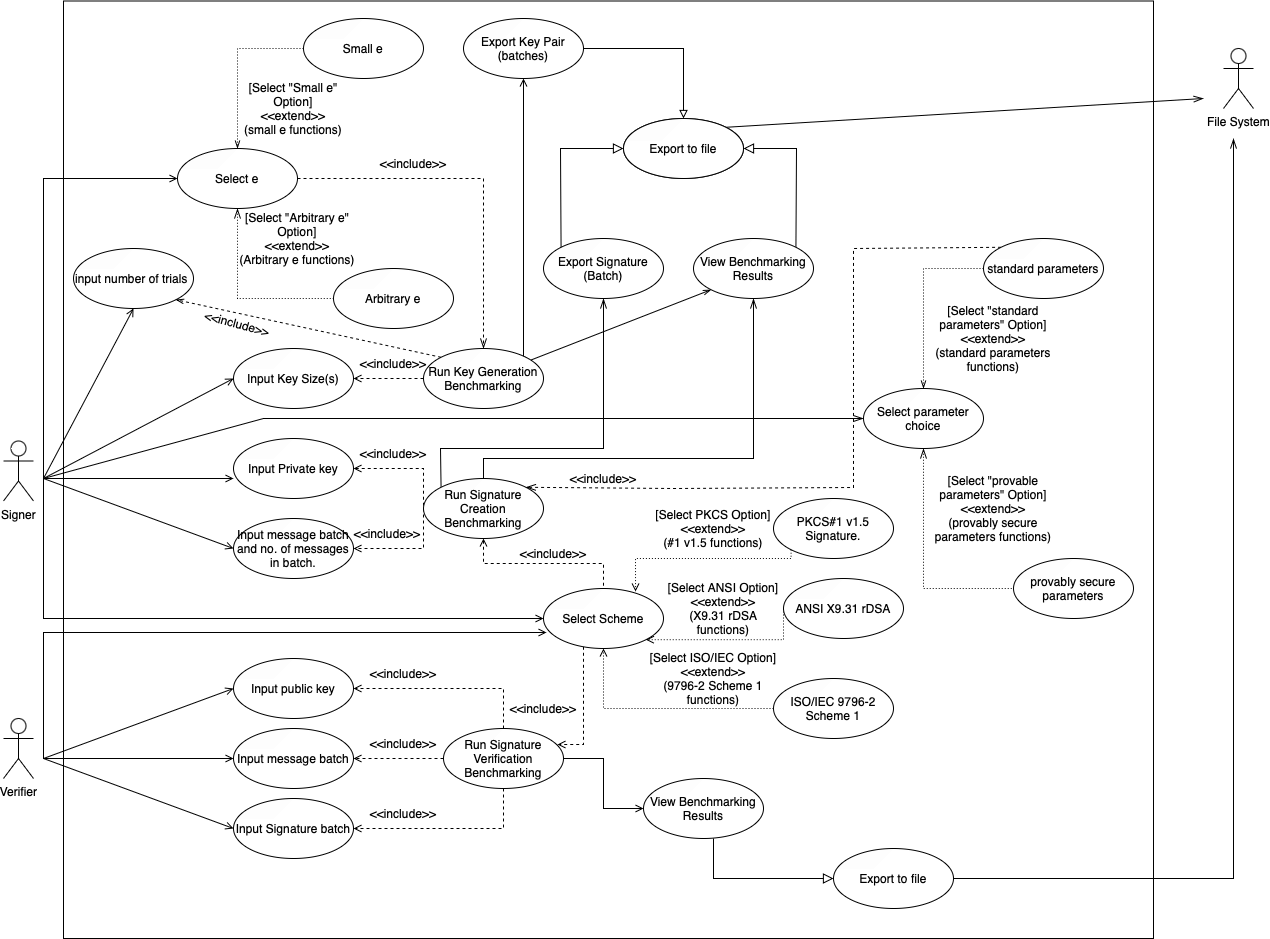
\includegraphics[scale=0.38]{poc_pictures/MAIN_USE-CASE.png}
    \caption{UML Use Case Diagram}
    \label{fig:uc}
\end{figure}



\textbf{Generate Keys Use Case}

\noindent\textbf{Flow of Events:}
\begin{enumerate}
    \item User selects "Generate Key" from the main menu options panel.
    \item User is presented with an input box prompting for the number of keys desired to be generated.
    \item User inputs desired number of keys into the box.
    \item System processes the request and updates the screen with the corresponding of number input boxes displayed vertically down the screen.
    \item System updates the screen with a checkbox labelled small e adjacent to each dynamically generated input box for each key.
    \item User inputs desired key sizes into each of the dynamically generated input boxes, additionally selecting the adjacent "small e" checkbox next to each input box where applicable.
    \item User is presented with an input box labelled enter number of trials for benchmarking run.
    \item User inputs desired number of trials into the box.
    \item System processes the request and completes the benchmarking run for the key generation process.
      \item System displays benchmarking results and notification informing the user that benchmarking process is complete.
      \item User is presented with options ”Export to file” for the most recently benchmarked private key and public key batches.
        \item User is presented with options ”Export to file” for benchmarking results.
        \item User selects desired options for exporting.
\end{enumerate}

\noindent\textbf{Alternative flows:}
\begin{enumerate}
    \item[3a.] User inputs an invalid number of keys.
    \begin{enumerate}
        \item[3a1.] System warns user about the invalid input and prompts them to enter a valid number of keys.
    \end{enumerate}
        \item[4a.] System encounters an error during process of displaying the dynamically generated input boxes.
    \begin{enumerate}
        \item[4a1.] System displays an error message and prompts the user to try again.
    \end{enumerate}
    \item[6a.] User inputs an invalid key size into one of the dynamically generated input boxes.
    \begin{enumerate}
        \item[6a1.] System warns user about the invalid input and prompts them to enter a valid key size .
    \end{enumerate}
     \item[8a.] User inputs an invalid number of trials.
    \begin{enumerate}
        \item[8a1.] System warns user about the invalid input and prompts them to enter a valid number of trials.
    \end{enumerate}
        \item[9a.] System encounters an error during benchmarking of the key generation creation process.
    \begin{enumerate}
        \item[9a1.] System displays an error message and resets screen back to initial view.
    \end{enumerate}  
\end{enumerate}



\textbf{Create Signature Use Case}

\noindent\textbf{Flow of Events:}
\begin{enumerate}
    \item User selects "Sign message" from the main menu options panel.
    \item User is presented with text boxes labeled "Input Private Key batch", "Input Message batch" and "Input no. of message".
    \item User provides all required inputs.
    \item User selects the desired signature scheme(s) to be used for benchmarking run from options ("PKCS\#1 v1.5 Signature", "ANSI X9.31 rDSA", ISO\slash IEC 9796-2 scheme 1).
        \item User selects the desired choice parameters to instantiate the chosen signature scheme(s) for benchmarking run from options ("standard parameters", "provably secure parameters").
  \item System processes the request and completes the benchmarking run for the signature creation process.
      \item System displays benchmarking results and notification informing the user that benchmarking process is complete.
      \item User is presented with options ”Export to file” for the resulting batch of computed signatures.
       \item User is presented with options ”Export to file” for benchmarking results.
       \item User selects desired options for exporting.
\end{enumerate}

\noindent\textbf{Alternative flows:}
\begin{enumerate}
    \item[3a.] User inputs an invalid or mismatched private key batch.
    \begin{enumerate}
        \item[3a1.] System warns user about the invalid input and prompts them to enter a valid private key batch.
    \end{enumerate}
     \item[3b.] User inputs an invalid or mismatched message batch.
    \begin{enumerate}
        \item[3b1.] System warns user about the invalid input and prompts them to enter a valid message batch.
    \end{enumerate}
     \item[3c.] User inputs an invalid number of messages.
    \begin{enumerate}
        \item[3c1.] System warns user about the invalid input and prompts them to enter a valid number of messages.
    \end{enumerate}
    \item[6a.] System encounters an error during benchmarking of the signature creation process.
    \begin{enumerate}
        \item[6a1.] System displays an error message and prompts the user to try again.
    \end{enumerate}
    \item[8a.]  User selected ISO\slash IEC 9796-2 scheme 1 in step 4.
    \begin{enumerate}
        \item[8a1.] User is presented with options "Export to file" for the computed batch of signatures and additionally if applicable a computed batch of non recoverable messages portions.
    \end{enumerate}
\end{enumerate}

\textbf{Verify Signature Use Case}

\noindent\textbf{Flow of Events:}
\begin{enumerate}
    \item User selects "Verify Signature" from the main menu options panel.
    \item User is presented with text boxes labeled "Input public Key batch", "Input Message batch" and "input signature batch".
    \item User provides all required inputs.
       \item User selects the desired signature scheme(s) to be used for benchmarking run from options ("PKCS\#1 v1.5 Signature", "ANSI X9.31 rDSA", ISO\slash IEC 9796-2 scheme 1).
         \item System processes the request and completes the benchmarking run for the signature verification process.
      \item System displays benchmarking results and notification informing the user that benchmarking process is complete.
      \item User is presented with options ”Export to file” for the results of signature verification for each and every message.
       \item User is presented with options ”Export to file” for benchmarking results.
       \item User selects desired options for exporting.
\end{enumerate}

\noindent\textbf{Alternative flows:}
\begin{enumerate}
    \item[3a.] User inputs mismatched or incorrect information.
    \begin{enumerate}
        \item[3a1.] System warns user about the incorrect input and suggests rechecking the inputs.
    \end{enumerate}
    \item[5a.] System encounters an error during verification.
    \begin{enumerate}
        \item[5a1.] System displays an error message and prompts the user to try again.
    \end{enumerate}
    \item[7a.]  User selected an ISO\slash IEC 9796-2 scheme in step 2.
    \begin{enumerate}
        \item[7a1.] The results of signature verification for each and every message in file offered for export, contains text corresponding to recovered portion of message if corresponding signature on message verified correctly.
    \end{enumerate}
\end{enumerate}

\subsection{Acceptance Tests}


\textbf{1. Benchmarking Key Pair Generation:}
\begin{enumerate}
\item Launch the benchmarking application and select "Generate Key" from the main menu.
\item Ensure the application presents an input box for entering the desired number of key pairs for generation.
\item Verify that after inputting the desired number of key pairs, the application dynamically displays corresponding input boxes for each key pair, along with a checkbox labeled 'small e' adjacent to each input box.
\item Check the functionality for the user to input desired key sizes into each dynamically generated input box and the option to select the 'small e' checkbox where applicable.
\item Confirm that the application presents an input box for entering the number of trials for the benchmarking run.
\item Test the process of inputting the desired number of trials and verify that the system processes the request correctly.
\item Inspect the system's ability to complete the benchmarking run for the key generation process without errors or exceptions.
\item Ensure the application displays benchmarking results along with a notification confirming the completion of the benchmarking process.
\item Verify the availability and functionality of the options to export both the most recently benchmarked private and public key batches, as well as the benchmarking results to a file.
\end{enumerate}


\textbf{2. Benchmarking Signature Generation:}
\begin{enumerate}
\item Locate the signature generation section in the application.
\item Use the browse option to provide a message batch.
\item Use the browse option to provide a valid private key batch.
\item If empty message batch or an invalid private key batch is provided, the user is informed to try again. 
\item selects a choice of parameters from options ("standard parameters", "provably secure parameters").
\item Ensure no errors or exceptions are displayed during the benchmarking of the signature creation process.
\item Check that the application notifies the user upon successful completion of the benchmarking process.
\item Verify options to export both the generated signatures and benchmarking results to a file.
\end{enumerate}

\textbf{3. Benchmarking Digital Signature Verification:}
\begin{enumerate}
\item Locate the signature verification section in the application.
\item Use the browse option to provide a message batch.
\item Use the browse option to provide a valid public key batch.
\item If empty message batch or an invalid public key batch is provided, the user is informed to try again.  
\item Ensure no errors or exceptions are displayed during the benchmarking of the signature verification process.
\item Check that the application notifies the user upon successful completion of the benchmarking process.
\item Verify options to export both the generated signature verification results and benchmarking results to a file.
\end{enumerate}



\textbf{4. Benchmarking Signature and Verification with PKCS#1 v1.5:}
\begin{enumerate}
\item Select the PKCS#1 v1.5 Signature Scheme for benchmarking within the application.
\item Conduct benchmarking of both the signature generation and verification processes with corresponding test batches using the previous steps. Ensure both processes succeed.
\item Verify the functionality to export the benchmarking results for both signature generation and verification processes to a file.
\item Verify the functionality to export the results for the actual verification of signatures to a file.
\end{enumerate}


\textbf{5. Benchmarking Signature and Verification with ANSI X9.31 rDSA:}
\begin{enumerate}
\item Select the ANSI X9.31 rDSA Signature Scheme for benchmarking within the application.
\item Conduct benchmarking of both the signature generation and verification processes with corresponding test batches using the previous steps. Ensure both processes succeed.
\item Verify the functionality to export the benchmarking results for both signature generation and verification processes to a file.
\item Verify the functionality to export the results for the actual verification of signatures to a file.
\end{enumerate}


\textbf{6. Benchmarking Signature Generation with ISO/IEC 9796-2:2010 Scheme 1:}
\begin{enumerate}
\item Set the application to use the ISO/IEC 9796-2:2010 Signature Scheme 1.
\item Locate the signature generation section in the application.
\item Use the browse option to provide a message batch.
\item Use the browse option to provide a valid private key batch.
\item If empty message batch or an invalid private key batch is provided, the user is informed to try again. 
\item selects a choice of parameters from options ("standard parameters", "provably secure parameters").
\item Ensure no errors or exceptions are displayed during the benchmarking of the signature creation process.
\item Check that the application notifies the user upon successful completion of the benchmarking process.
\item Verify options to export both the generated signatures and benchmarking results to a file.
\item Verify options to export a batch of messages to a file (e.g., as a message recovery mode, non recoverable portion of messages is transmitted along with signature).
\end{enumerate}

\textbf{7. Benchmarking Signature Verification with ISO/IEC 9796-2:2010 Scheme 1:}
\begin{enumerate}
\item Select the ISO/IEC 9796-2:2010 Scheme 1 for benchmarking within the application.
\item Conduct benchmarking of both the signature verification process with corresponding test batches using the previous steps. Ensure both processes succeed.
\item Verify the functionality to export the benchmarking results for the signature verification process to a file.
\item Verify the functionality to export the results for the actual verification of signatures to a file.
\item Check that results for the actual verification of signatures additionally contain recovered message portions.
\end{enumerate}


\section{Appendix B.2 Design}
\subsection{Program packages}
\begin{figure}[H]
    \centering
    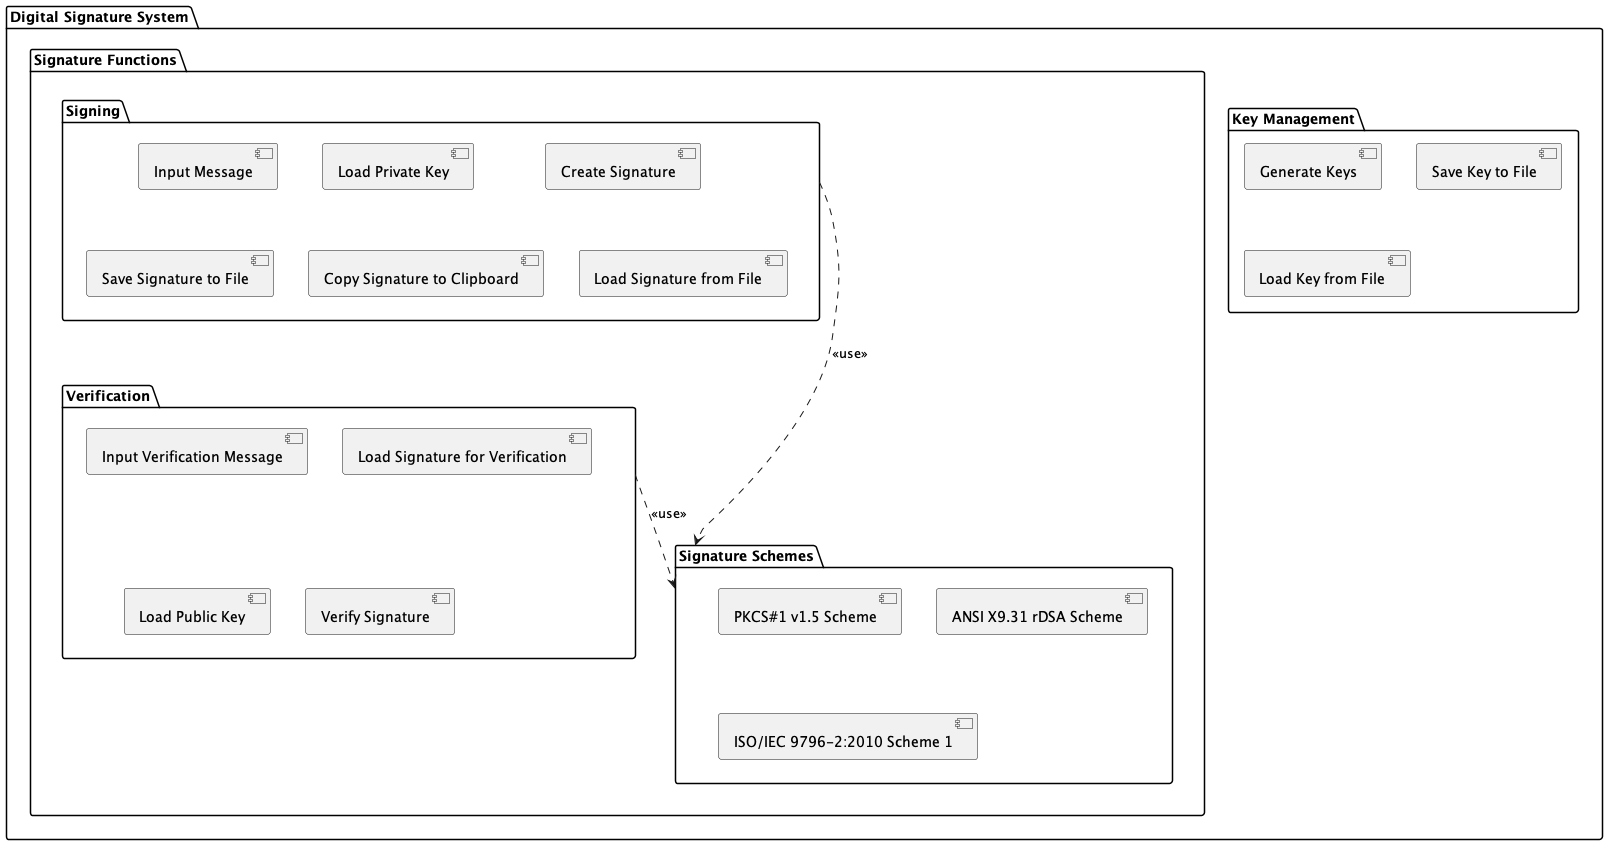
\includegraphics[scale=0.31]{poc_pictures/package.png}
    \caption{POC program Packages}
    \label{fig:pack}
\end{figure}
Figure \ref{fig:pack} depicts the core functionality of the POC program and is in direct alignment with previously elaborated on (see requirements) user activities of signing, creating keys, and verifying, using a specified scheme like PKCS\#1-v1.5.
\subsection{UML sequence diagram}
\begin{figure}[H]
    \centering
    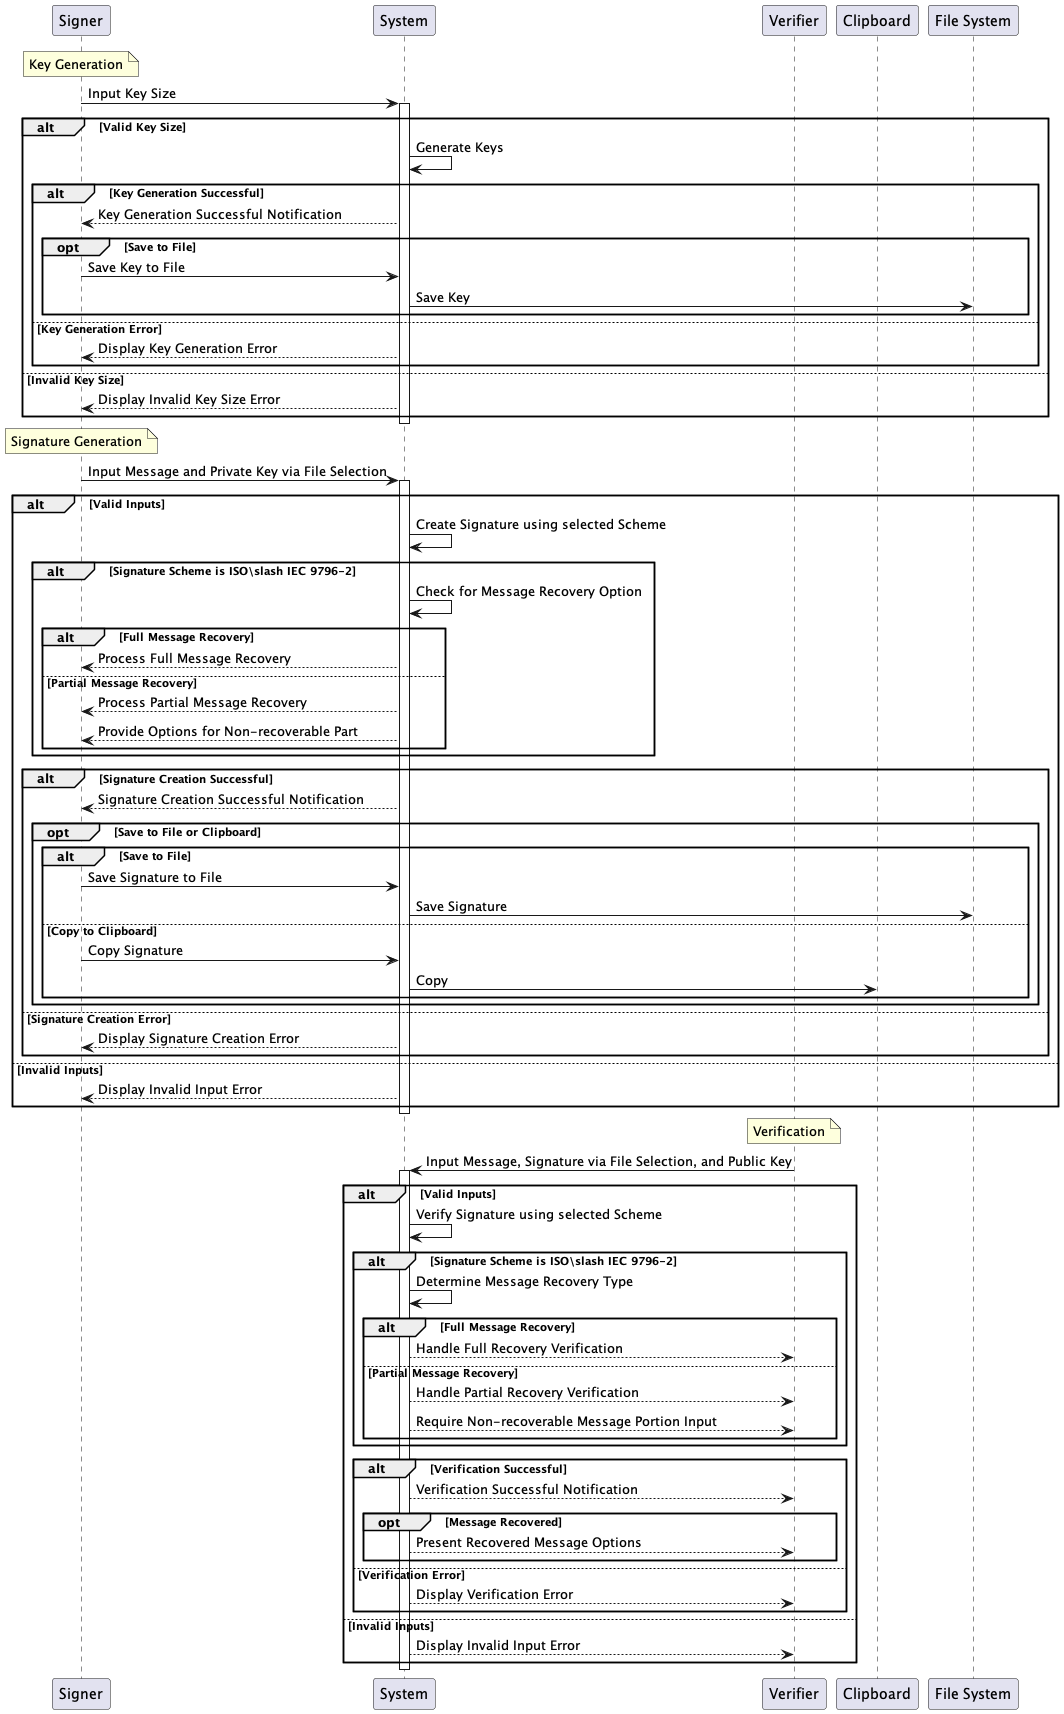
\includegraphics[scale=0.38]{poc_pictures/sequenceV2.png}
    \caption{UML Sequence Diagram}
    \label{fig:uc}
\end{figure}
The above diagram is mostly a high level view of the core behaviour that can be expected to performed by a user of the proof of concept of program. The point at which the diagram departs from this, is the specialised functionality related to the message recovery signature schemes of the ISO standard. These schemes require special consideration because their behaviour differs from the standard digital signature process. The ISO/IEC 9796-2 schemes incorporate message recovery features, where part or all of the original message can be reconstructed from the signature itself. This necessitates additional logic in both the signing and verifying processes. 

For partial message recovery, the signer needs to manage the non-recoverable portion of the message, ensuring that it is correctly returned alongside the signature. Subsequently they may then input the non-recoverable portion as part of their interaction with the verification process in attempt to recover the remaining portion of message. 

For full message recovery, the entire message is embedded in the signature, eliminating the need for a separate message input during verification but requiring careful handling to extract and validate the message from the signature. 

These nuances demand specialised user interfaces and system checks, making the ISO schemes distinct in their interaction and processing requirements within the application.

Initially, the user is prompted to generate cryptographic keys, providing a key size that, if valid, leads to the creation of a private and public key pair. The user can then opt to save these keys onto their file system.

Once keys are in place, the user can sign a message. They input the message into the system and load their private key. If the inputs are correct, the system employs a chosen signature algorithm to create a digital signature, which the user can save or copy to their clipboard. In case of invalid input or an error during signature creation, the user is informed with an error message.

For verification, the user inputs a message, loads the digital signature and the corresponding public key. The system checks the signature against the message using the public key. If the signature is valid, a success notification is displayed; otherwise, the user is alerted to a verification error. Throughout this process, the system guides the user with notifications or error messages based on the success or failure of the operations performed.


 

\section{Appendix B.3 Testing}

\subsection{Appendix B.3A Integration Testing}
My approach towards integration testing was tailored to ensure that each of the application modules functioned correctly within their respective Model-View-Controller (MVC) frameworks. Utilising TestFX \cite{TestFX2023}, a testing framework for JavaFX applications, the testing concentrated on the internal workings of each module, examining how well the MVC components within a single module interacted with each other.

The first step of this testing was to ensure that the main controller effectively managed transitions from the application-level main menu into the different functional modules. This is the only form of inter-module communication that the application utilises.

The primary role of TestFX in this scenario was to automate interactions within each module, testing the cohesion between the Model, View, and Controller layers. For example, in the key generation module, TestFX helped ensure that the user input in the View layer was accurately processed by the Controller, and the resulting data was correctly managed and reflected by the Model. This pattern was replicated in the signature module that encapsulates the signature creation and verification functionalities as well.



\subsection{Appendix B.3B System Testing}
In the context of this proof of concept, my approach to system testing has been intentionally focused and concise, targeting primarily the core functional requirements. Understanding that exhaustive testing is not the goal at this stage, I concentrated on verifying the key operations that are crucial for my application: key generation, signature creation, and signature verification.

During the system testing phase, I employed a targeted strategy, prioritising Critical Path Testing. This involved ensuring that the essential functions of the application – generating keys, creating signatures, and verifying them – performed accurately under normal use scenarios. Alongside this, I conducted Happy Path Testing to confirm that the application behaves as expected in ideal conditions.

Given the scope of this project, comprehensive testing for errors and edge cases was not a primary focus. However, I did engage in some basic Negative Testing to ensure that the system could handle common user input errors gracefully. This approach provided me with a sufficient level of confidence in the application's operational integrity and usability, particularly for a proof of concept.

\begin{comment}
The results from this phase have been succinctly documented, with an emphasis on the performance of the application's key features. These findings are instrumental in my initial evaluation of the system's feasibility and highlight potential areas for further development in subsequent iterations." 
\end{comment}



\begin{table}[H]

  \centering

  \label{tab:table1}
  \resizebox{\textwidth}{!}{%
    \begin{tabular}{|l|p{1.5cm}|p{1.8cm}|p{2.5cm}|p{3.5cm}|p{2.3cm}|}
      \hline
      \textbf{Type of
Testing} & \textbf{Module Scope} & \textbf{Goal of tests} & \textbf{Test Objective} & \textbf{Technique} & \textbf{Completion Criteria}\\
      \hline
      Functional Testing  & All Modules. & The goals of these tests are to verify acceptance of data, its retrieval, and the correct adoption of requirement related logic & Ensure entry and retrieval of data along expected navigation of an application & Execute function, using valid/invalid data, ensuring:
\begin{itemize} \item When valid /invalid data is inputted, respectively, the expected results occur, or corresponding error message is displayed.
\item Each requirement is met. \end{itemize} & All planned tests have been executed\\
     
      \hline
    \end{tabular}%
  }
\end{table}


\begin{table}[H]
   \caption{\textbf{Main Menu Test Cases}}
  \centering
  \label{tab:table1}
  \resizebox{\textwidth}{!}{
    \begin{tabular}{|l|p{2.5cm}|p{2.5cm}|p{2.5cm}|p{2.5cm}|p{3.5cm}|}
      \hline
      \textbf{Test ID} & \textbf{Prerequisites} & \textbf{Test Steps} & \textbf{Test Data} & \textbf{Expected Result} & \textbf{Actual Result}\\
      \hline
      MainMenu-001 & Application is launched and the user is presented with the main menu. & 
      \begin{enumerate}
      \item Click on the "[K] Generate Keys" button.
      \end{enumerate} & N/A & The application should navigate to the key generation page without errors. & Pass \\
      \hline
      MainMenu-002 & Application is launched and the user is presented with the main menu. & 
      \begin{enumerate}
      \item Click on the "[S] Sign Document" button.
      \end{enumerate} & N/A & The application should navigate to the signature creation page without errors. & Pass \\
      \hline
      MainMenu-003 & Application is launched and the user is presented with the main menu. & 
      \begin{enumerate}
      \item Click on the "[V] Verify Signature" button.
      \end{enumerate} & N/A & The application should navigate to the signature verification page without errors. & Pass \\
      \hline
    \end{tabular}%
  }
\end{table}

\begin{longtable}{|l|p{2.5cm}|p{2.5cm}|p{2.5cm}|p{2.5cm}|p{3cm}|}
  \caption{\textbf{Key Generation Test Cases}}
  \hline
  \textbf{Test ID} & \textbf{Prerequisites} & \textbf{Test Steps} & \textbf{Test Data} & \textbf{Expected Result} & \textbf{Actual Result} \\
  \hline
  KeyGen-001 & Application is installed and operational; the user is on the Key Generation page. & 
  \begin{enumerate}
  \item Navigate to the "Generate Keys" section.
  \item Enter a valid bit size in the input field.
  \item Click the "Generate Keys" button.
  \end{enumerate} & 1024, 1024 & The system should generate a key pair using the specified bit sizes without errors. & Pass \\
  \hline
  KeyGen-002 & Application is installed and operational; the user is on the Key Generation page. & 
  \begin{enumerate}
  \item Navigate to the "Generate Keys" section.
  \item Enter a string of special characters in the input field.
  \end{enumerate} & @\#\%\&*[(\$ & The system should not accept the input and display an error message indicating that only numerical bit sizes are valid & Pass \\
  \hline
  KeyGen-003 & Application is installed and operational; the user is on the Key Generation page. & 
  \begin{enumerate}
  \item Navigate to the "Generate Keys" section.
  \item Enter an excessively long string of numbers in the input field.
  \item Click the "Generate Keys" button.
  \end{enumerate} & A string of numbers exceeding normal bit size lengths (e.g., 1000 digits). & The system should reject the input and display an error message indicating that the bit size is too long and not valid. & \textcolor{red}{Fail.} \\
  \hline
  KeyGen-004 & Application is installed and operational; the user is on the Key Generation page. & 
  \begin{enumerate}
  \item Navigate to the "Generate Keys" section.
  \item Enter alphanumeric characters in the input field.
  \item Click the "Generate Keys" button.
  \end{enumerate} & abc123 & The system should not accept the input and should display an error message that only numeric values are valid. & Pass \\
  \hline
  KeyGen-201 & Application is installed and operational; the user has successfully generated keys using the "Generate Keys" feature. & 
  \begin{enumerate}
  \item After key generation, click on the "Export Private Key" button.
  \item Check the application's default save location for the presence of the new signature file.
  \end{enumerate} & N/A (The action uses the application's UI) & The signature file is automatically saved to the default location specified by the application. The file should contain the correct signature data, formatted as expected for a digital signature. & Pass \\
  \hline
\end{longtable}








\begin{longtable}{|l|p{2.5cm}|p{2.8cm}|p{2cm}|p{2cm}|p{2cm}|}
  \caption{\textbf{Signature Creation Test Cases}} \label{tab:signature_creation} \\
  \hline
  \textbf{Test ID} & \textbf{Prerequisites} & \textbf{Test Steps} & \textbf{Test Data} & \textbf{Expected Result} & \textbf{Actual Result} \\
  \hline
  \endfirsthead

  \multicolumn{6}{c}{\textbf{Table \ref{tab:signature_creation} (continued): Signature Creation Test Cases}} \\
  \hline
  \textbf{Test ID} & \textbf{Prerequisites} & \textbf{Test Steps} & \textbf{Test Data} & \textbf{Expected Result} & \textbf{Actual Result} \\
  \hline
  \endhead

  \hline
  \multicolumn{6}{r}{\textit{Continued on the next page}} \\
  \endfoot

  \hline
  \endlastfoot

  Sign-001 & User is on the "Sign" page of the application. & 
  \begin{enumerate}
    \item Click the "Import Text..." button.
    \item Select a valid text file to import for signing.
    \item Verify that the text box is replaced with the name of the imported file and a green checkmark is displayed.
    \item Click the "Import Private Key" button and select a valid private key.
    \item Choose a signature scheme from the dropdown menu if available.
    \item Click "Create Signature".
  \end{enumerate} & Valid text file for import, valid private key file. & The application should successfully complete the signature generation process & Pass.  Screen transitions to notification panel with success message \\
  \hline
  Sign-002 & User is on the "Sign" page of the application without any key or text pre-loaded. & 
  \begin{enumerate}
    \item Manually enter text into the "ENTER TEXT TO SIGN:" field.
    \item Click "Create Signature" without importing a private key.
  \end{enumerate} & "Example text to sign" & The application should prompt the user to import a private key before allowing the signature creation to proceed. & Pass. Error pop-up informing input must be provided for all fields is displayed \\
  \hline
  Sign-003 & User is on the "Sign" page of the application. A valid private key is already imported. & 
  \begin{enumerate}
    \item Click the "Import Text..." button.
    \item Select an invalid file format or a corrupted text file.
    \item Attempt to create a signature.
  \end{enumerate} & Invalid or corrupted file. & The application should display an error message indicating the file is not valid for import. & Pass. File chooser limits choice of file to be imported to text files.\\
  \hline
  Sign-004 & User is on the "Sign" page with a valid text and scheme selected. & 
  \begin{enumerate}
    \item Click "Import Private Key" and select an invalid or corrupted private key file.
    \item Attempt to sign the message.
  \end{enumerate} & Invalid or corrupted private key file. & The application should display an error message indicating the private key file is not valid for import. & \textcolor{red}{Fail.} \\
  \hline
      Sign-005  & User is on the "Sign" page with a valid text, and private key imported & 
  \begin{enumerate}
    \item Attempt to create a signature without choosing a signature scheme.
  \end{enumerate} &
  & The application should display an error message indicating signature scheme needs to be selected. & Pass \\
    \hline
  Sign-Export-001 & User has attempted to create a digital signature but the process failed due to an invalid key or other errors. & 
  \begin{enumerate}
    \item Attempt to click on the "Export Signature" or "Copy to Clipboard" button after a failed signature creation attempt.
  \end{enumerate} & N/A (The action uses the application's UI) & The application should either disable the export/copy functionality & Pass. Error pop-up informing input must be provided for all fields is displayed, so screen does not transition to panel where export/copy functionality is provided.  \\
  \hline
  Sign-Export-002 & User has successfully created a digital signature on the "Sign" page. & 
  \begin{enumerate}
    \item After signature creation, check for any UI indication that the signature is ready to be exported (such as a confirmation message or an enabled "Export" button).
    \item If a confirmation message or similar indicator is part of the design, confirm its presence.
    \item Proceed with the export or copy operation as designed.
  \end{enumerate} & N/A (The action uses the application's UI) & Any UI indicators or messages that should appear post-signature creation to guide the user to export or copy the signature should be present and correct according to the application design. & Pass. Screen transitions to notification panel with success message and export/copy functionality provided \\
  \hline
  Sign-Export-003 & User has successfully created a digital signature on the "Sign" page. & 
  \begin{enumerate}
    \item After signature creation, click on the "Export Signature" button.
    \item Wait for the application to perform the export operation automatically.
    \item Check the application's default save location or the location indicated by the application for the presence of the new signature file.
    \item Open the signature file with a text editor to verify that it contains the correct signature data.
  \end{enumerate} & N/A (The action uses the application's UI) & The signature file is automatically saved to the default location specified by the application. & Pass. File saved to same directory application was run in.  \\
  \hline
\end{longtable}





\begin{longtable}{|p{1.2cm}|p{3cm}|p{3cm}|p{4cm}|p{4cm}|}
  \caption{\textbf{Verification Test Cases}} \label{tab:verification_test_cases} \\
  \hline
  \textbf{Test ID} & \textbf{Prerequisites} & \textbf{Test Steps} & \textbf{Expected Result} & \textbf{Actual Result} \\
  \hline
  \endfirsthead

  \multicolumn{5}{c}{\textbf{Table \ref{tab:verification_test_cases} (continued): Verification Test Cases}} \\
  \hline
  \textbf{Test ID} & \textbf{Prerequisites} & \textbf{Test Steps} & \textbf{Expected Result} & \textbf{Actual Result} \\
  \hline
  \endhead

  \hline
  \multicolumn{5}{r}{\textit{Continued on the next page}} \\
  \endfoot

  \hline
  \endlastfoot

   Verify-002 & User is on the "Verify" page of the application with no files pre-loaded. & 
  \begin{enumerate}
    \item Manually input text into "ENTER TEXT TO VERIFY:".
    \item Click "Import Public Key".
    \item Select a valid public key file.
    \item Manually input a signature into "ENTER SIGNATURE:".
    \item Select the appropriate signature scheme, if applicable.
    \item Click "Verify Signature".
  \end{enumerate}
  & The application should accept manual input and the imported public key, perform verification on "Verify Signature" click, and display the result. & Pass. Screen transitions to notification panel with result of verification. \\
  \hline
  Verify-003 & User is on the "Verify" page of the application. & 
  \begin{enumerate}
    \item Attempt to import an invalid or corrupted text file by clicking "Import Text...".
    \item Attempt to verify the signature.
  \end{enumerate}
  & The application should display an error message indicating the file is not valid for import. & Pass. File chooser limits choice of file to be imported to text files. \\
  \hline
  Verify-004 & User is on the "Verify" page with a valid text and signature imported. & 
  \begin{enumerate}
    \item Click "Import Public Key" and select an invalid or corrupted public key file.
    \item Attempt to verify the signature.
  \end{enumerate}
  & The application should display an error message indicating the public key file is not valid for import. & Pass. \\
      \hline
    Verify-005 & User is on the "Verify" page with a valid text, signature imported and public key imported & 
  \begin{enumerate}
    \item Attempt to verify the signature without choosing a signature scheme.
  \end{enumerate}
  & The application should display an error message indicating signature scheme needs to be selected. & \textcolor{red}{Fail.} \\

\end{longtable}
\subsection{Bug Report}
 \begin{longtable}{|p{2.5cm}|p{1.7cm}|p{3.1cm}|p{2.5cm}|p{2.5cm}|p{2.5cm}|}
  \caption{\textbf{Bug Report Table}} \label{tab:bug_report} \\
  \hline
  \textbf{Bug ID} & \textbf{Test ID} & \textbf{Test Steps} & \textbf{Expected Result} & \textbf{Actual Result} & \textbf{Solution} \\
  \hline
  \endfirsthead

  % Repeat the header on the next pages
  \multicolumn{6}{c}%
  {{\bfseries Table \thetable\ continued from previous page}} \\
  \hline 
  \textbf{Bug ID} & \textbf{Test ID} & \textbf{Test Steps} & \textbf{Expected Result} & \textbf{Actual Result} & \textbf{Solution} \\
  \hline
  \endhead

  \hline
  \multicolumn{6}{|r|}{{Continued on next page}} \\ 
  \hline
  \endfoot

  \hline
  \endlastfoot

 Bug-001 Key Generation causes application crash when a number that exceeds what can be accepted as an integer is inputted Bit  causes crash . & KeyGen-003 &
\begin{enumerate}
\item Navigate to "Generate Keys".
\item Enter 11111111111.
\item Click "Generate Keys".
\end{enumerate} & System should reject input and display error for long bit size. & Fail: System crashes. & Catch and handle exception thrown by Integer.parseInt call so that error is displayed as intended \
\hline
Bug-002 Invalid or Corrupted Private Key File causes crash& Sign-004 &
\begin{enumerate}
\item On "Sign" page, click "Import Private Key".
\item Select an invalid or corrupted private key file.
\item Attempt to sign the message.
\end{enumerate} & Error message indicating invalid private key file. & Fail: System crashes. &  Correct regex pattern used to identify regex pattern so that error is displayed as intended \
\hline
Bug-003 Not selecting signature causes application crash & Verify-005 &
\begin{enumerate}
\item On "Verify" page, import valid text, signature, and public key.
\item Attempt to verify without selecting a signature scheme.
\end{enumerate} & Error message for not selecting a signature scheme. & Fail: System crashes. & Modify check for signature scheme drop value to use "!=" to check for equality with null rather than .equals(). \
\hline

\end{longtable}


\chapter{Appendix C Diary}

\textbf{Diary Entry: Week of 18th - 24th September 2023}

This week was dedicated to writing a first draft of the abstract for my project (PKCS signature scheme) and researching arbitrary precision arithmetic for a library I may look to implement as part of the aims for the project

On Monday, I started writing about its importance, touching on its widespread use and history.
Tuesday was a continuation, emphasising why it's such a vital system.

By Wednesday, I added details on potential security issues, particularly focusing on something
called the Bleichenbacher attacks. I was initially puzzled about how these attacks affected the
signature scheme.

On Thursday and Friday, after more research, I figured out the difference between how these attacks
affect encryption and signature aspects of the system. This helped clarify some of my earlier
confusion.

Over the weekend, I added insights on why, despite some concerns, many still prefer the PKCS system.
I also touched upon a new research finding that supports its use. By Sunday, I detailed my main
goals for this project, hoping to create a useful tool that compares different signature schemes.

Next I will clarify whether I should consider implementing a self-made big number library as part of
the project and hopefully advance significantly in the creation of the project plan.

\textbf{Diary Entry - Week of 25th September - 1st October 2023}

Met with my supervisor for initial meeting. Discussed potential extensions to the original project
specifications and in general what the project entails. Refocused and refined the project plan,
emphasising deterministic RSA hash-and-sign schemes, especially PKCS\#1 v1.5. Made structural changes
to the introduction and abstract, enhancing clarity. Set up the Maven project directory on GitLab
and further developed the project timeline. Transitioned all documentation from Microsoft Word to
latex, drafting the literature review in the process. By week's end, automated referencing in latex
for enhanced efficiency.

\textbf{Diary Entry - Week of 2nd October - 8th October 2023}

This week, I refined and expanded the Risks and mitigation section, established a risk
quantification table, and deepened my understanding of digital signature schemes. The literature
review for the interim report was integrated, and significant progress was made in drafting the
cryptographic foundation of the report. By the weekend, focus was channeled into classifying digital
signature schemes and laying out a clear structure for detailed exploration of specific signature
schemes in upcoming sessions. Next I will begin writing the introductory section on digital
signatures for my report.

\textbf{Diary Entry - Week of 9th October - 15th October 2023}

I Started the week with supervisor meeting, confirming my focus on the POC PKCS Signature for term 1
and was given advice to potentially using the top 1000 English words for the signature program when
I sought guidance on the type of data I could provide to be signed. I delved into textbook RSA,
highlighting its vulnerabilities. By Friday, I had expanded on RSA's role in digital signatures,
introducing potential attacks and Hashed RSA signatures. The weekend saw me laying the foundation
for all three schemes considered in the project by formally defining them. I then began to explore
the motivation of provably secure signature schemes.

\textbf{Diary Entry - Week of 16th October - 22nd October 2023}

I started the week attempting to try and understanding trapdoor permutations, especially how they
tie into RSA. Following this I began work on enumerating the requirements for the proof of concept
program. By the end Friday, I had detailed the user stories and actors for the program with a
corresponding a UML use case diagram. During the weekend I first focussed on expanding the
motivation for provable security section with subsections on real world implications and
limitations. I finished off the week on Sunday by trimming down the report to make it more concise.

\textbf{Diary Entry - Week of 23rd October - 29th October 2023}

The week started with a meeting where I received constructive feedback on my project plan,
specifically that I had spent too much time on PKCS\#1 v1.5 encryption scheme and Bleichenbacher
attacks, which were deemed beyond the project’s scope. We clarified the implications of the interim
report's word limit, and I was reassured that my report’s structure was on the right track, though I
was advised against including full software design documents.

I primarily focused on refining my project plan based on feedback. After restructuring my report and
creating an appendix for the software requirements of the proof of concept program, I turned my
attention to conceptualising and beginning the implementation of the RSA key generation process,
culminating in a complete first draft by Friday. The weekend was dedicated to initiating a new
chapter on security proof in the report, laying down the foundational concepts and starting to weave
them into the project's larger narrative.

\textbf{Diary Entry - Week of 30th October - 5th November 2023}

Focused on enhancing the clarity and structure of my project report, I began by unifying the
background concepts for security proofs. I refined the introduction, dividing it into clear aims and
objectives. I then pruned excess information from several sections for brevity and clarity,
particularly around RSA concepts. I started work on the design phase for the proof of concept
program kicking off with a draft outline of the MVC architecture and factory patterns, which I later
formalised into a UML class diagram. By the week's end, I finalised design diagrams, integrated them
into the report, and refined the section on provable security. The upcoming weeks are now poised for
the implementation stage.

\textbf{Diary Entry - Week of 6th November - 12th November 2023}

This week, I had the 4th meeting with my supervisor, where we clarified the required content for the
security proofs in my report, focusing on the practical implications for the signature schemes. My
progress on the interim report was positively noted, and I announced my intention to submit a draft
shortly. I began conceptualising (Wednesday) and then coding the PKCS\#1 v1.5 signature scheme (
Thursday) with a focus on modularity. By the end of the week, I had not only implemented this scheme
but also completed the security proof chapter of my report, emphasising the implications for
practical parameter choices. I also improved the key generation process to be more parametrisable,
setting a foundation for term 2 work where this is required.

\textbf{Diary Entry - Week of 13th November - 19th November 2023}

This week, I focused on implementing various signature schemes, starting with conceptualising and
drafting the ANSI X9.31 signature scheme. Using Test-Driven Development, I developed and refined
this implementation, leveraging the modular code structure from the earlier PKCS scheme.

A significant part of the week involved troubleshooting and resolving issues related to signature
verification. In the ANSI implementation, legitimate signatures occasionally failed to verify. The
problem was traced to the message encoding method and was fixed by adjusting the first padding byte.

When implementing the ISO/IEC 9796-2 scheme, I encountered a similar issue with signature
verification failures. This time, it was due to the first padding byte causing the encoded message's
big integer representation to sometimes exceed the modulus size, leading to verification failures.
After thorough research and comparison with open-source implementations, I realised the necessity of
prepending an initial 0x00 byte to the encoded message array, a Java-specific implementation detail.

The week concluded with a substantial refactoring of the ISO scheme's class structure, simplifying
it to a single class that automatically adjusts the recovery mode based on the user's message
length.

\textbf{Diary Entry - Week of 20th November - 26th November 2023}

This week, I made substantial progress in both my report and the development of the proof of concept
program. I sent a draft of my report to my supervisor and rescheduled our meeting to Friday for
feedback. I then focused on developing models for the proof of concept program, beginning with the
key generation model and applying the state design pattern effectively. By midweek, I completed all
essential models for the program, setting the stage for controller development.

I then moved on to developing the program's views, ensuring they supported the observer design
pattern, and completed the implementation of all application views. After receiving positive
feedback and suggestions for minor improvements on my report from my supervisor, I advanced to
developing the controllers, completing the GenController and initiating the SignatureController.

Over the weekend, I finished the SignatureController, integrating it seamlessly with the views, and
developed the MainController to manage the application flow. The application was functionally
complete, albeit pending more rigorous testing. I concluded the week by reorganising the project and
code directory to better reflect the MVC pattern and separate different functional modules.


\textbf{Diary Entry - Week of 27th November - 3rd December 2023}

This week, I focused on finalising my project for the interim submission I started with integration
testing for the mainMenu and Sign view features using TestFX, ensuring the UI and
model-view-controller interactions worked correctly. By Tuesday, I had completed all integration
testing, including tests for the verify view, and updated the appendix with detailed test cases.

Midweek, I shifted to preparing my project presentation, developing introductory slides and key
concept overviews. During this period, I also enhanced the JavaDoc documentation across the project
and detailed the system testing results in the appendix.

On Friday, I create a new launch class for the application and generated a fat jar containing the
full application (with all classes and dependencies needed to run it). Additionally, I started
recording demo videos for the presentation and the final project submission.

Over the weekend, I put the finishing touches on the presentation slides and the demo videos. I also
updated the project's README with detailed run instructions and refined the report to incorporate
specifics from my implementation of the signature schemes.

Next, I will organise everything in a manner appropriate for the final submission and clean up any
remaining loose ends, ensuring that all elements of the project are polished.
%%%% ADD YOUR BIBLIOGRAPHY HERE
\newpage

\addcontentsline{toc}{chapter}{Bibliography}
\printbibliography
\label{endpage}
\end{document}

\end{article}
